% !TeX TS-program = txs:///latexmk | txs:///view-log | txs:///view-pdf | txs:///convert
\documentclass{article}

\usepackage{tikzducks}

%
%\tikzset{
%shape example/.style= {color = black!30,
%draw,
%fill = yellow!30, line width = .5cm, inner xsep = 2.5cm, inner ysep = 0.5cm}
%}


\begin{document}

% normal duck

\begin{tikzpicture}
	\duck{Gold}
\end{tikzpicture}
%
% grumpy
\begin{tikzpicture}
	\grumpyduck{Gold}
\end{tikzpicture}
%
% blue duck

\begin{tikzpicture}
	\duck{SteelBlue}
\end{tikzpicture}

% female

\begin{tikzpicture}
	\duck{Gold}
	\addlonghair{SeaGreen}
\end{tikzpicture}
%
% alien duck

\begin{tikzpicture}
	\duck{Gold}
	\addalien{LimeGreen}
\end{tikzpicture}
%
% hat duck

\begin{tikzpicture}
	\duck{Gold}
	\addhat{SaddleBrown}
\end{tikzpicture}

% sunglasses

\begin{tikzpicture}
	\duck{Gold}
	\addsunglasses{black!50!brown}{black}
\end{tikzpicture}
%
% icecream

\begin{tikzpicture}
	\duck{Gold}
	\addicecream{Wheat}{Orchid}{Chocolate}
\end{tikzpicture}
%
% samcarter

\begin{tikzpicture}
	\duck{Wheat!95!red}
	\addjacket{MidnightBlue}
	\addlonghair{OrangeRed!50!Brown}
\end{tikzpicture}

% unicorn

\begin{tikzpicture}
	\duck{MediumVioletRed!35!white}
	\addlonghair{MediumVioletRed}
	\addunicorn{MediumVioletRed}
\end{tikzpicture}
%
% short hairs

\begin{tikzpicture}
	\duck{Wheat}
	\addtshirt{LightBlue!50!white}
	\addjacket{LightSlateGrey}
	\addshorthair{brown!50!Grey}
\end{tikzpicture}
%
% Men in black
\begin{tikzpicture}
	\grumpyduck{Wheat}
	\addtshirt{white}
	\addjacket{black}
	\addtie{black}
	\addhat{black}
	\addsunglasses{black}{black}
\end{tikzpicture}

% prof. van duck
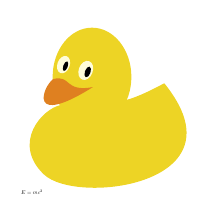
\begin{tikzpicture}
	\duck{Gold!40!white}
	\makeeinstein{gray!50!white}
	\addglasses{brown!70!black}
	\addbook{brown!70!black}{\scalebox{0.2}{$E=mc^2$}}
\end{tikzpicture}
%
% Knuth
\begin{tikzpicture}
	\makeknuth
\end{tikzpicture}
%
% for the counter wizard Christian Hupfer

\begin{tikzpicture}
	\duck{Gold}
	\addwizzard{BlueViolet!50!Pink}{Gold}
\end{tikzpicture}

% Brazil colour duck for Paulo

\begin{tikzpicture}
	\definecolor{brazilgreen}{RGB}{0,155,58}
	\definecolor{brazilyellow}{RGB}{254,223,0}
	\definecolor{brazilblue}{RGB}{0,39,118}
	\duck{brazilyellow}
	\addjacket{brazilblue}
	\addshorthair{brazilgreen}
\end{tikzpicture}
%
% swimming

\begin{tikzpicture}
	\addwater{cyan!50!blue}
	\duck{Gold}
\end{tikzpicture}
%
% ducklings
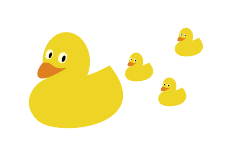
\begin{tikzpicture}[scale=0.6]
	\duck{Gold}
	\begin{scope}[xshift=90pt, scale=.3, yshift=150pt]
		\duck{Gold}
	\end{scope}
	\begin{scope}[xshift=60pt, scale=.3, yshift=100pt]
		\duck{Gold}
	\end{scope}
	\begin{scope}[xshift=80pt, scale=.3, yshift=50pt]
		\duck{Gold}
	\end{scope}		
\end{tikzpicture}

\end{document}
